\section{Waffle}
\label{sec:3-instr}

% Done: The key idea is that I should talk about my solution to the program with more details.
% Done: I have explained that there is another way of resolving the problem.
% Now it's time to explain what is the difference in the guidance defined in Waffle
% Definitions?!:
% Resource complexity, Overall resource complexity (ERU), Elites, Visitors
% OR: Shared memory, instrumentation, fuzzing

% Tasks
% -T1: Explain the way AFL works
% -T2: Explain an overview of the additional properties added to AFL by Waffle

\begin{figure}[!t]
  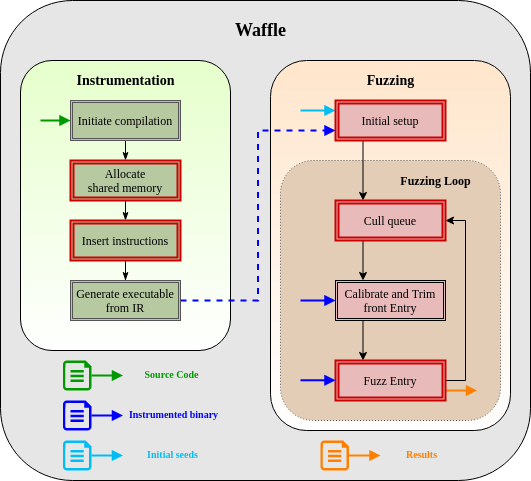
\includegraphics[width=0.8\textwidth]{Chapter3/waffle-proc.png}
  \centering
  \caption{Fuzzing phases of Waffle. The red rectangles specify the changed components.}
  \label{fig:waffle-phases}
\end{figure}

The exponential search space for different inputs with a specific behavior, such as a crash or hang, is approached by evolutionary algorithms of AFL to investigate the possible inputs for producing such events. AFL leverages on code coverage, file size, and execution time to guide the genetic algorithm to maintain the cases which discover more regions of the code, in a practically fast fasion. Waffle exploits the coverage-guided findings to discover regions of code, and tries to increase resource usages through the evolution.

% -T: Explain the waffle-proc.png

As illustrated in Figure \ref{fig:waffle-phases}, Waffle has major modifications on AFL in instrumentation and fuzzing phases. The shared memory is designed to be capable of storing the \textit{resource complexity} of an execution. Waffle also extends AFL's Coverage Pass to collect performance features. In the fuzzing phase, the fuzzer evaluates code coverage and resource usage of the executions (\texttt{cull\_queue}), and considers a fitness for each of the generated entries. Next, the front entry in the queue of entries is passed to the fuzzing loop for testing, and the loop continues before a termination signal. In the following sections we inspect the changes made in AFL to introduce Waffle.

\subsection{Resource complexity of execution}

% ?   #########################################################################
% -T: What the resource complexity is and how it is measured

To address resource usage of an execution, we estimate the engaged resource usage of executions. Waffle does not analyse the source code for finding the resource complexities, such as time and space complexity; however, it records the resource consuming instructions. For instance, an instruction such as \texttt{memcpy} takes CPU usage (and time) for its execution, and may access the program's available memory. To bring in the involved instructions in a complete run of a program, Waffle presume a set of instructions and monitors the occurrences. A trace of the envolvement of the instructions is stored in the shared memory for the need of fuzzing.

% ?   #########################################################################
% -T1: Estimated Resource Usage

We define the \textbf{Estimated Resource Usage} (shortened to ERU) of an application as \textit{an estimation of the resources required to execute a program}. This definition follows the program's performance based on the effort for completing an execution. To calculate the ERU of a program in a concrete execution, each of the instructions using the \textit{engaging resources} is monitored. (e.g. \texttt{memcpy} instructions)  

% ?   #########################################################################
% -T1: How waffle uses the ERU through entire fuzzing chain

Waffle replicates AFL's coverage-discovery techniques with modifications to calculate and leverage ERU for performance-guidance. While fuzzing the inputs, ERU of the executions is stored in an array of the same size as AFL's coverage map, and for each hit on the coverage map, Waffle updates the same index of it's performance array (As a result, the hitmaps of both of the arrays are the same, and they both can represent the code-coverage). The target index is calculated by tracing the taken edge on the program's CFG. In AFL, a favored entry points to an input which suggests something \textit{interesting}, that is, a better code coverage or a faster (and with a smaller input size) execution. Furthermore, Waffle finds the \textit{favor} in any entry which is either coverage-guided (better code coverage) or performance-guided (more exhaustive execution).

% !     Subsection 1: Instrumentation
\subsection{Instrumentation}
\label{subsec:inst}

% ?   #########################################################################
% -T1: Generally define and explain the added and modified modules in Instrumentation

The \texttt{llvm-mode} subproject under Waffle's directory contains the recipe for building a clang-based compiler with the aforementioned instrumentations. The resulting compiler, i.e. \texttt{./waffle-clang}, has the capability for inserting the guidance-instructions into the program. Waffle initiates the compilation by locating the shared memory to pass the measurements out of execution's procedure. Waffle includes an (extra to AFL) array of 4-bytes integers for tracking the ERU of each basic block. As a result, Waffle requires $5\times2^{16}=320KBs$ of memory space in addition to the genuine program's memory consumption (Listing \ref{lst:wafl-rt}). Correspondingly, instrumented program leaves a trace of the ERUs (collected by the \textit{visitor} functions) of the basic blocks on array of ERUs. After the initial configurations for instrumentation, the compilation recipe is applied to the compilation procedure, and the generated compiler follows the instructions (as seen in psudocode \ref{lst:hash}) for instrumentation during the compilation of any given source code.

\begin{lstlisting}[language=C++,style=CodeStyle,label={lst:hash},caption={Select element and update in shared\_mem}]
  counter = lg(count_instructions())
  cur_location = <COMPILE_TIME_RANDOM>;
  edge = cur_location ^ prev_location;

  cov_shared_mem[edge]++;
  per_shared_mem[edge]+=counter;

  prev_location = cur_location >> 1;
\end{lstlisting}
  
\lstinputlisting[language=C,style=CodeStyle,float=tb,label={lst:wafl-rt},caption={LLVM instrumentation initialization - \texttt{\_\_wafl\_area\_ptr} is the region that is allocated for instruction counters}]{Codes/Chapter3/waffle-llvm-rt.o.c}  

% ?   #########################################################################
% -T1: Explain LLVM visitor functions
% -T2: Explain the implementation of the visitor functions

\subsubsection{Visitors}

The implementation of \textit{LLVM's instruction visitor functions} \cite{inst_visitor} helps Waffle in searching and counting the instances of the instructions used in an execution. LLVM provides functions for \texttt{getting} and \texttt{setting} the instructions in a range of the code section of program. Listing \ref{lst:visitors} shows an example of how Waffle uses the visitor counters; the exampled member function \texttt{visitInstruction(Instruction \&I)} checks if an instruction is of \textbf{any} type - which can be set to detect other specific types, such as \texttt{memcpy} - and Waffle uses an instance of the class \texttt{CountAllVisitor} containing the occurrences of (any) instructions in a specific range of the code section. As mentioned before, this code section is selected from the first instruction of a basic block, to the last instruction before leaving the according basic block.

\lstinputlisting[language=C++,style=CodeStyle,label={lst:visitors},caption={Visitors example}]{Codes/Chapter2/visitor.cpp}

% ?   #########################################################################
% -T1: Explain the procedure of the module pass 

Listing \ref{lst:llvm-pass} shows a snippet of Waffle's Module Pass procedure. In line 6, a pointer to the shared array is introduced to the scope of the program. After this initial setup, Waffle digs into the basic blocks and creates an instance of the \texttt{CountAllVisitor} struct. By passing the current basic block to the visitor module, the result of the counting is returned and is stored in \texttt{CAV} variable.

\lstinputlisting[language=C,style=CodeStyle,label={lst:llvm-pass},caption={LLVM-mode instrumentation pass}]{Codes/Chapter3/mini-wafl-llvm-pass.so.cc}

% -T1: Explain why the log function is used

The linear increment in \texttt{CAV} has a relatively large variance for the counters in each basic block. For instance, if Waffle chooses to count all instructions in an execution, the basic blocks contributed an average of $18$ instructions for the ERU \footnote{Tested C++ implementations of QuickSort, MergeSort, and DFS}. To prevent overflows of the ERU cells in long executions, Waffle maintains the logarithm of each counter (Equation \ref{eq:log}). This modified counter is then set as a constant value for increasing the corresponding edge-index of the ERU array (Formula \ref{eq:ERU-log}). It is noticeable that the content of each cell may be increased by more than one edge; this is caused by the conflicts in the hashing procedure of edges.

\begin{equation}
  \label{eq:log}
  CNT = \log_{2}^{CAV+1}
\end{equation}

\begin{equation}
  \label{eq:ERU-log}
  ERU[edge] += \sum_{visit} \log_{2}^{CAV_{visit}+1} \approx \sum_{visit} \log_{2}^{CAV_{visit}} = visits \times \log_{2}^{CAV_{visit}}
\end{equation}

% ?   #########################################################################

% -T1: Explain how the instrumentation is applied

After applying the above recipe for instrumentation, the obtained \texttt{waffle-clang} compiler is then used for generating an executable with the mentioned features. To use this compiler, the following command creates the binary file we are looking for:

\begin{lstlisting}[language=bash,style=CommandStyle,label={lst:wafl-clang}]
  ./waffle-clang target.c -o instr_target.bin
\end{lstlisting}

% !   Subsection 2: Fuzzing

\subsection{Fuzzing}

% !   #########################################################################
% !                You need to change it as illustration changed
% !   #########################################################################

% -T: Explain the waffle-fuzz-proc illustration

\begin{figure}[!b]
  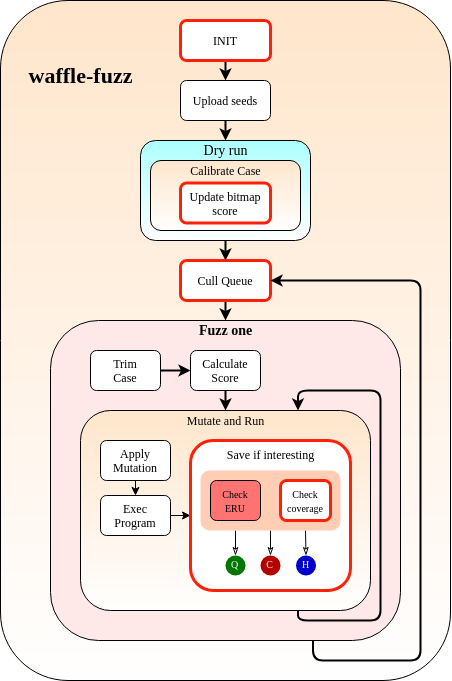
\includegraphics[width=0.8\textwidth]{Chapter3/waffle-fuzz-proc.png}
  \centering
  \caption{Waffle fuzzer: The red rectangles specify the new or changed components.}
  \label{fig:waffle-fuzz-proc}
\end{figure}

Waffle follows the same fuzzing procedure as AFL's, with some modifications in processing the inputs, and selecting next inputs to fuzz. As illustrated in Figure \ref{fig:waffle-fuzz-proc}, Waffle initializes the procedure by introducing new variables to the entries of the queue, as well as the changes to the \texttt{top\_rated} array of entries. Next, after uploading the seeds, a dry run is performed on the provided seeds for fuzz testing, and the \texttt{top\_rated} entries are updated to establish a measurement for selecting a favored input for testing. Followingly, the fuzzing loop starts by an initial culling of the queue, modifying the priorities of the entries by comparing the execution features tracked in \texttt{top\_rated}, i.e. the coverage and performance features, and finally starts fuzzing the selected entry of queue. \texttt{fuzz\_one} function (\textbf{Fuzz one} box in Figure \ref{fig:waffle-fuzz-proc}), accepts a queue entry and tests the program with mutations of the corresponding input file. The next major modification in our fuzzer, is submitted in the procedure of saving an interesting input (\texttt{save\_if\_interesting}). This function now considers the performance values, and an input with either an interesting coverage-based or ERU-based performance, is saved for future fuzzing. By running the function \texttt{save\_if\_interesting} on each of the input files returned from mutation, either a new queue entry (\textbf{Q}), crash (\textbf{C}), or hang (\textbf{H}) is produced and the corresponding input is stored in an associated directory. This function, \texttt{save\_if\_interesting}, also updates the bitmap scores (\ref{lst:wafl-update-score}) and reevaluates the \texttt{top\_rated} entries.

\lstinputlisting[language=C,style=CodeStyle,float=tb,label={lst:wafl-update-score},caption={\texttt{update\_bitmap\_score}: Waffle ignores the fav\_factor in case of a long lasting execution}]{Codes/Chapter3/waffle-fuzz/update_bitmap_score.c}

% -T: Explain the data structures used and developed for fuzzing

Waffle initiates the tracing arrays for both coverage (\texttt{trace\_bits}) and ERU (\texttt(trace\_ERU)). These arrays have the same structure as mentioned in the previous subsection (\ref{subsec:inst}). The structure of \texttt{queue\_entry}'s is changed by adding two new variables, \texttt{TERU}, for tracking the summation of the ERUs after executing a test entry, and a normalized version of TERU as $nTERU= \lfloor \log_{2} {TERU}\rfloor$. On the other hand, the \texttt{top\_rated} array which tracks the winners of each edge, is extended to maintain both the coverage and the performance winners (Figure \ref{fig:waffle-top_rated}). To better understand this approach, we explain the functionality of \texttt{cull\_queue()} as shown in Listing \ref{lst:cull-queue}.

If an entry shows an interesting coverage behavior, it updates the \texttt{top\_rated} array, controlled by the cells under the entry's coverage map; if a cell on \texttt{trace\_bits} is showing a better coverage, the first pointer of \texttt{top\_rated} is changed to the current entry (which is already stored in the queue of entries). If there is no interests in the code-coverage, Waffle assesses \texttt{TERU} of the \texttt{queue\_entry}, and updates the lower (second) index of \texttt{top\_rated} array by comparing the current \texttt{TERU} with \texttt{TERU}s of the pointed entries stored in \texttt{top\_rated}.

\begin{figure}[!b]
  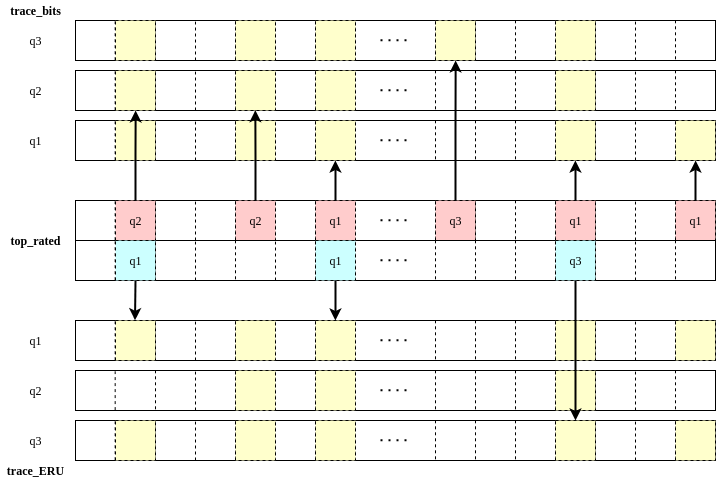
\includegraphics[width=0.8\textwidth]{Chapter3/waffle-top_rated.png}
  \centering
  \caption{\texttt{top\_rated} array: Waffle keeps track of the relevant coverage and performance features}
  \label{fig:waffle-top_rated}
\end{figure}

% -T: Cull queue

Waffle adds any entry with a coverage-related or ERU-related benefit, to the queue of entries. Later, when it is time to select an entry for fuzzing, Waffle culls the queue as shown in Listing \ref{lst:cull-queue}. Each element of \texttt{top\_rated} list is either empty, or is pointing to a queue's entry. Waffle iterates on the \texttt{top\_rated} entries, and as shown in the code, it first checks if it can detect a new code coverage in a cell index $i$ (lines 18 to 25), otherwise, the fuzzer tries the ERU for a new discovery. In lines 26 to 34, for the same index $i$, if \texttt{top\_rated[i][1]} is available and it is not \textit{visited} before, then every other \texttt{top\_rated[j][1]} with the same approximated \texttt{nTERU}, for $j$ in the range of indices, is set as \textit{visited} and is skipped in this iteration. This approach helps the fuzzer to set at least one entry with the same \texttt{nTERU}, if it was not tagged as a coverage-guiding test case, and is introducing a distinct execution with a specific \texttt{nTERU}. This technique helps the fuzzer to find the most beneficial test cases in the queue, and ignore the obsolete ones.

\lstinputlisting[language=C,style=CodeStyle,label={lst:cull-queue},caption={Waffle \texttt{cull\_queue}}]{Codes/Chapter3/waffle-fuzz/cull_queue.c}

% -T: Fuzz one

After the queue was culled, the first favored entry of the queue is selected for fuzzing. First, Waffle keeps the \textit{trimming} procedure the same as AFL's, and does not consider the changes in the \texttt{ERUs[]} while trimming the case. This is because of the fact that the trimming procedure maintains the values of the \texttt{trace\_bits[]} to remain the same, and as a result, the \texttt{ERUs[]} remain the same, and as a result there is no need to check this array. Before getting into the mutation loop, Waffle determines the effort it wants to take for fuzzing the current case, and calculates \texttt{perf\_score} for this purpose (same as AFL's).

% -T: Mutation (not modified), Execution

In both deterministic and havoc stages of mutation, fuzzer executes the program on new files and stores them if they expose interesting information. An input is interesting if i) it generates an input based on the heuristics for guidance, to generate corrupted executions, ii) a crash is occured, or iii) a hang is occured. The results in (ii) and (iii) do not need any modification in our work. Waffle generates inputs and examines them to verify if they show a \textit{new coverage}, or they expose an exhaustive execution. The main goals of Waffle are to guide the code coverage to explore, as well as generating resource exhaustive executions. Listing \ref{algo:waffle-save-if-interesting} presents a pseudocode of \textit{save\_if\_interesting}. The function \texttt{is\_exhaustive()} aggregates the values of the \texttt{ERUs[]} and if the execution increases the current maximum ERU, the test case for this performance is picked as \textit{interesting} (Listing \ref{lst:is-exhaustive}).

% ! Add an appendix for save_if_interesting

\begin{algorithm}
    \KwIn{\textbf{$in-memory test case$}}
    CALL has\_new\_bits RETURNING hnb\;
    \textcolor{green}{CALL has\_better\_elite RETURNING hbe}\;
    \If{hnb or hbe}{
        SAVE case to file\;
    } 
    \caption{save\_if\_interesting}
    \label{algo:ifi-waffle}
\end{algorithm}

\lstinputlisting[language=C,style=CodeStyle,label={lst:is-exhaustive},caption={Find the interest based on the execution's resource usage}]{Codes/Chapter3/waffle-fuzz/is_exhaustive.c}
